\documentclass[uplatex]{jsarticle}
\usepackage[dvipdfmx]{graphicx}
\usepackage{amsmath}
\begin{document}
\begin{flushright}
  鈴木理也
\end{flushright}

\setcounter{section}{1}
Chapter2
\section{二階線形微分方程式}

\subsection{Problem set 2.4}
\large
1.初期値問題(4)${y_0},{v_0}$を初期値とした周期運動を見つける。
$  \omega_0=\pi,y_0=1$とする 
  $$ my'' + ky =0$$ 
  $$ {\lambda}^2 +\frac{k}{m} = 0 \leftrightarrow {\lambda} = \pm i {\sqrt{\frac{k}{m}}}$$ 
  ${\omega_0}={\sqrt{\frac{k}{m}}}$とすると

  $$ y(t) = A cos({\omega_0}t) + B sin({\omega_0}t) $$
${y_0}$から始まり${v_0}$が初期速度なので

\begin{align}
  y_0 &= A cos(0 * \pi) + B sin(0* \pi) \notag \\
  y_0 &= A = 1 
\end{align}

微分して

\begin{align}
  y'(t) &= -{\omega_0} A sin({\omega_0}t) + {\omega_0} B cos({\omega_0}t) \notag \\
  v_0 &= -{\omega_0}A sin 0 + {\omega_0}B cos 0 \notag \\
   &= -{\omega_0}A*0 + {\omega_0}B*1 \notag \\
   &= {\omega_0}B \notag \\
  B &= \frac{v_0}{\omega_0} 
\end{align}
A,Bを入れると、こうなる。
$$ y(t) = cos({\omega_0}t) + \frac{v_0}{\omega_0} sin({\omega_0}t) $$
式の$v_0$を0,負、正とするとグラフはこうなる。


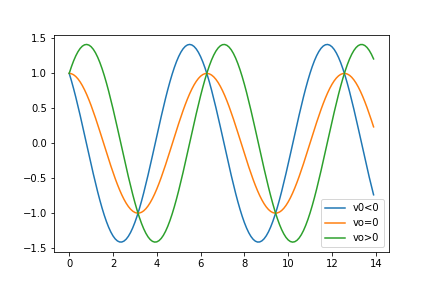
\includegraphics{./hertz.png}



2. 重さ20nt、バネを2cm伸ばした。調和振動と周期。
$$ W = 0.02k $$

$$ k = \frac{W}{0.02}= \frac{20}{0.02} = 1000kg/sec^2 $$

$$ m = \frac{W}{g}= \frac{20}{9.8} \approx 2.04(kg) $$

$$ f = \frac{\omega_0}{2\pi} = \frac{\sqrt{\frac{k}{m}}}{2\pi} \frac {\sqrt{\frac{1000}{2.4}}}{2\pi} = \frac{\sqrt{490.19}}{2\pi} \approx 3.52(Hz)$$


3. 重さを2倍にしたときと、バネを二倍にしたとき



*重さが2倍の場合
$$ f = \frac{\omega}{2\pi} $$
$$ \omega = \sqrt{\frac{k}{m}}$$
$$ \omega_1 =\sqrt{\frac{k}{2m}} = \frac{1}{\sqrt{2}}* \sqrt{\frac{ k}{m}}= \frac{1}{\sqrt{2}}* \omega$$
$$ f_1 = \frac{\omega_1}{2\pi}= \frac{1}{\sqrt{2}}*f $$
$ \frac{1}{\sqrt{2}}$ 周期が遅くなる



*バネを二倍にした場合
$$ \omega_1 =\sqrt{\frac{2k}{m}} = \sqrt{2} \omega$$
$$ f_1 = \frac{\omega_1}{2\pi}= \sqrt{2}f $$
$ \sqrt{2} $ 周期が早くなる。


4. いいえ
$$ \frac{k}{m} に関係しないから$$
5. バネをいろいろ

$$ f = \frac{\omega}{2\pi} $$
1, $m=5kg,k_1=20 nt/m$の場合
\begin{align}
  f &= \frac{\sqrt{\frac{20}{5}}}{2\pi} \notag \\ 
    &= \frac{2}{2\pi} \notag  \\
    &= \frac{1}{\pi} \notag \\
    &\approx {0.318}Hz \notag  \\
\end{align}

2, $m=5kg, k_2 = 45 nt/m $の場合
\begin{align}
  f &= \frac{\sqrt{\frac{45}{5}}}{2\pi} \notag \\
    &=\frac{3}{2\pi} \notag \\
    &\approx{0.477}Hz \notag 
\end{align}

3, $k_1+ k_2$の場合
\begin{align}
  f &= \frac{\sqrt{\frac{k_1+k_2}{m}}}{2\pi} \notag \\ 
    &= \frac{\sqrt{\frac{20+45}{5}}}{2\pi} \notag \\ 
    &\approx{0.574}Hz \notag 
\end{align}
\end{document}
